\chapter{Analisis}
\label{chap:analisis}

\section{Analisis Sistem Kini}
\label{sec:analisiskini}
Pada halaman utama KIRI (dapat dilihat pada gambar \ref{fig:3_KIRI_main}), terdapat beberapa bagian yaitu:

\begin{figure}[H]
	\centering
	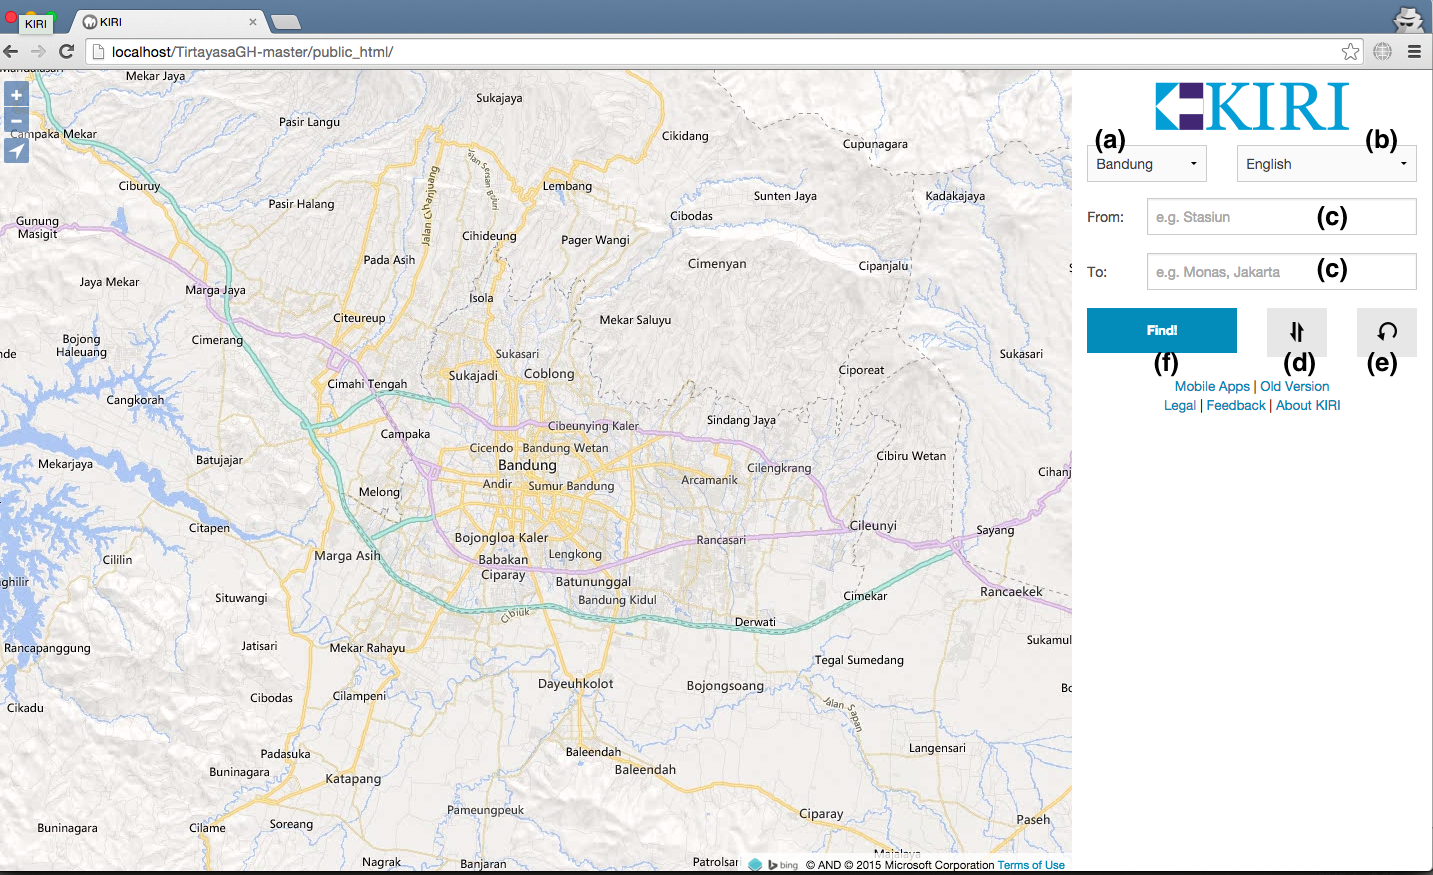
\includegraphics[scale=0.3]{Gambar/KIRI-main}
	\caption{Halaman Utama KIRI} 
	\label{fig:3_KIRI_main}
\end{figure}

\subsection{Peta}
Pada halaman utama KIRI (dapat dilihat pada gambar \ref{fig:3_KIRI_main}), terdapat beberapa bagian yaitu:
    \begin{enumerate}
    		\item \textbf{Peta}
    		\item \textbf{Form Samping} yang terdiri dari beberapa bagian, yaitu:
    		\begin{enumerate}
    			\item Dropdown Menu Kota
    			\item Dropdown Menu Bahasa
    			\item Textfield
    			\item Tombol Swap
    			\item Tombol Reset
    			\item Tombol Find
    		\end{enumerate}
    \end{enumerate}

\begin{figure}[H]
	\centering
	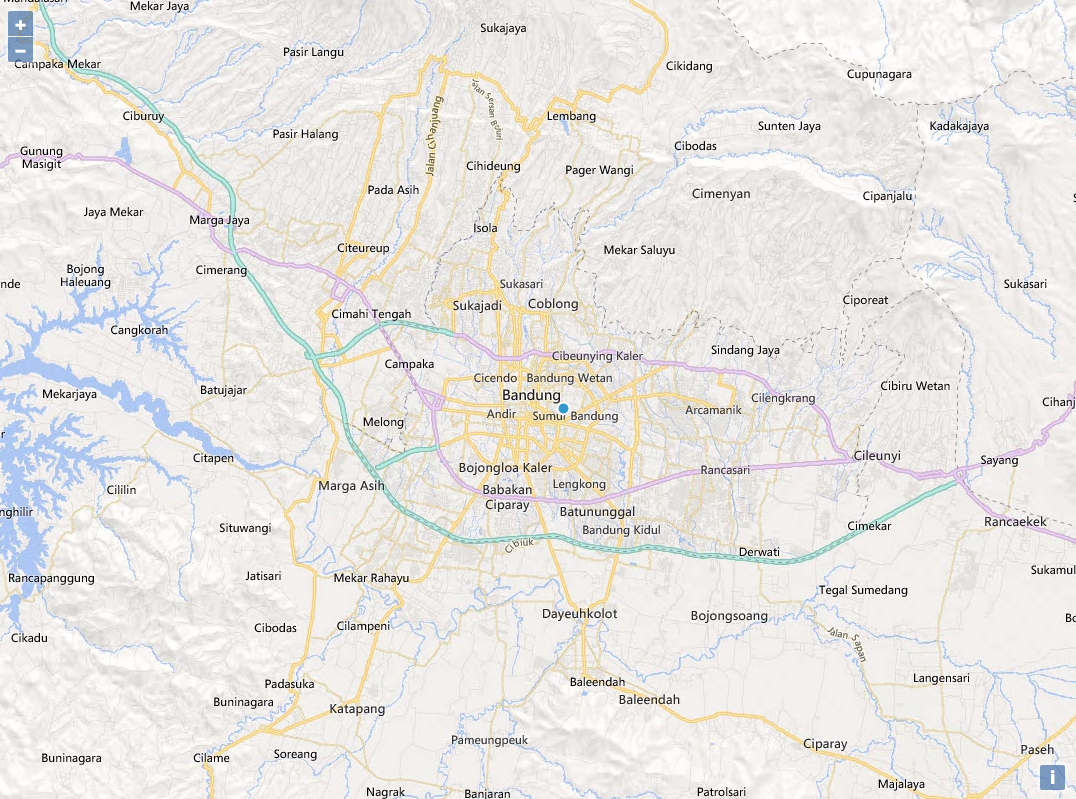
\includegraphics[scale=0.4]{Gambar/KIRI-peta}
	\caption{Peta pada KIRI} 
	\label{fig:3_KIRI_peta}
\end{figure}

KIRI menggunakan OpenLayers yang berbasis JavaScript untuk memuat peta pada halaman \textit{web}. Pertama melakukan deklarasi peta yang digunakan menggunakan BingMaps. Penggunaan BingMaps membutuhkan dua \textit{parameter}, yaitu \textit{key} yang merupakan kunci untuk menggunakan BingMaps dan \textit{imagerySet} yang merupakan tipe peta pada BingMaps. dan tipe peta pada BingMaps tersebut seperti pada kode listing \ref{lst_3_php_peta_bing}.

\begin{lstlisting}[caption=Deklarasi peta BingMaps,label = {lst_3_php_peta_bing}]
var mapLayer = new ol.layer.Tile(
{
	source : new ol.source.BingMaps(
	{
		key : 'AuV7xXD6_UMiQ5BLoZr0xkpjLpzWqMT55772Q8XtLIQeuDebHPKiNXSlZXxEr1GA',
		imagerySet : 'Road'
	})
});
\end{lstlisting}

%Untuk memunculkan tombol GPS Location yang berfungsi untuk pencarian lokasi berdasarkan lokasi pengguna. Pertama membuat elemen tombol dengan 

Untuk menambahkan fitur pada peta OpenLayers, seperti membuat marker pada peta dan membuat rute pada peta dapat dicapai dengan membuat objek ol.source.Vector seperti pada kode listing \ref{lst_3_php_peta_olvector}.

\begin{lstlisting}[caption=Objek ol.source.Vector,label = {lst_3_php_peta_olvector}]
var resultVectorSource = new ol.source.Vector();
var inputVectorSource = new ol.source.Vector();
\end{lstlisting}

Setelah deklarasi peta beserta konfigurasi fitur yang terdapat pada peta, memasukkan semua fitur pada \textit{layers} dan \textit{target} untuk memasukkan \textit{id tag} yang digunakan pada HTML seperti pada kode listing \ref{lst_3_php_peta_instansiasi}.

\begin{lstlisting}[caption=Instansiasi peta,label = {lst_3_php_peta_instansiasi}]
var map = new ol.Map(
	{
		...
		layers : [ mapLayer, new ol.layer.Vector({source: inputVectorSource}), new ol.layer.Vector({source: resultVectorSource}) ],
		target : 'map'
});
\end{lstlisting}

\subsection{Form Samping}
Form yang terdapat pada halaman utama KIRI (Gambar \ref{fig:3_KIRI_form}) terdiri dari:
\begin{figure}[H]
	\centering
	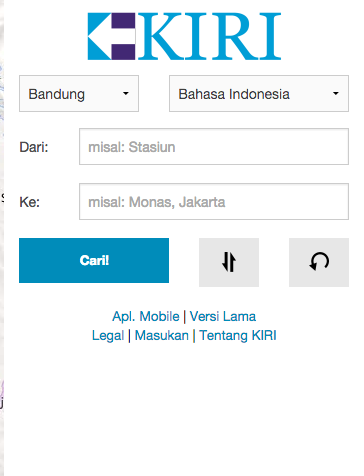
\includegraphics[scale=0.5]{Gambar/KIRI-form}
	\caption{Form pada KIRI} 
	\label{fig:3_KIRI_form}
\end{figure}

\subsubsection{Dropdown Menu Kota}
\textit{Dropdown} yang berfungsi untuk memilih kota yang akan ditampilkan pada peta (Gambar \ref{fig:3_KIRI_drop_kota}).

\begin{figure}[H]
	\centering
	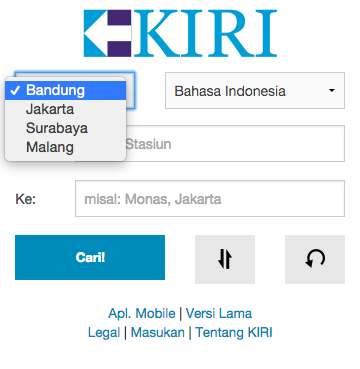
\includegraphics[scale=0.5]{Gambar/KIRI-drop-kota}
	\caption{Dropdown Menu Kota pada KIRI} 
	\label{fig:3_KIRI_drop_kota}
\end{figure}

Melakukan deklarasi variabel regioninfos sebagai \textit{associated array} pada file constants.php. Setiap kota direpresentasikan sebagai variabel proto\_region\_KOTA dimana KOTA adalah kota yang ada pada KIRI. Setiap proto\_region\_KOTA merupakan array dengan indeks:
\begin{enumerate}
	\item \textit{lat} sebagai garis lintang,
	\item \textit{lon} sebagai garis bujur,
	\item \textit{zoom} sebagai tingkat \textit{zoom} untuk memperbarui peta,
	\item \textit{name} untuk menampilkan pilihan kota,
	\item \textit{searchplace\_regex} untuk pencarian rute pada pilihan kota.
\end{enumerate} 
Kode dapat dilihat pada kode listing \ref{lst_3_php_dropdown_kota_regioninfos}.

\begin{lstlisting}[caption=Deklarasi variabel regioninfos,label = {lst_3_php_dropdown_kota_regioninfos}]
..
/** Different parameters for different regions. */
	$regioninfos = array(
		$proto_region_bandung => array(
			'lat' => -6.91474,
			'lon' => 107.60981,
			'radius' => 17000,
			'zoom' => 12,
			'searchplace_regex' => ', *(bandung|bdg)$',
			'name' => 'Bandung'
		),
		$proto_region_jakarta => array(
			'lat' => -6.21154,
			'lon' => 106.84517,
			'radius' => 15000,
			'zoom' => 11,
			'searchplace_regex' => ', *(jakarta|jkt)$',
			'name' => 'Jakarta'
		),
		$proto_region_surabaya => array(
			'lat' => -7.27421,
			'lon' => 112.71908,
			'radius' => 15000,
			'zoom' => 12,
			'searchplace_regex' => ', *(surabaya|sby)$',
			'name' => 'Surabaya'
		),
		$proto_region_malang => array(
			'lat' => -7.9812985,
			'lon' => 112.6319264,
			'radius' => 15000,
			'zoom' => 13,
			'searchplace_regex' => ', *(malang|mlg)$',
			'name' => 'Malang'				
		)
	);
..
\end{lstlisting}

Untuk menampilkan pilihan kota, pertama mengambil array regioninfos, lalu melakukan pengulangan sebanyak nilai yang terdapat pada regioninfos. Dalam pengulangan tersebut, menulis \textit{tag} HTML \verb!option! sesuai dengan \textit{name} yang terdapat pada regioninfos, jika \textit{name} tersebut sama dengan \textit{region} pengguna, maka opsi tersebut akan terpilih. Kode dapat dilihat pada kode listing \ref{lst_3_php_dropdown_kota_tampilan}

\begin{lstlisting}[caption=Menampilkan pilihan kota kepada pengguna ,label = {lst_3_php_dropdown_kota_tampilan}]
..
<select class="fullwidth" id="regionselect">
	<?php
		foreach ($regioninfos as $key => $value) {
			print "<option value=\"$key\"";
			if ($key == $region) {
				print " selected";
			}
			print ">" . $value['name'] . "</option>\n";
		}
	?>
</select>
..
\end{lstlisting}

Untuk memperbarui peta, KIRI menggunakan fungsi JavaScript dengan menerima dua parameter, yaitu newRegion dan updateCookie. Pertama membuat \textit{cookie} dengan kunci region, lalu membuat variabel \textit{point} dengan mengubah String menjadi LonLat dari titik tengah peta yang dituju. Untuk memperbarui peta dengan mengatur titik tengah pada peta yaitu memanggil \textit{method} \verb!setCenter! yang menerima parameter ol.proj.transform yang berisi garis lintang dan bujur serta kode dari Sistem  dan Transformasi  Koordinat. Setelah itu, mengatur tingkat \textit{zoom} dengan memanggil \textit{method} \verb!setZoom! dengan parameter berupa tingkat \textit{zoom} dari peta yang dituju. Kode dapat dilihat pada kode listing \ref{lst_3_php_dropdown_kota_update}

\begin{lstlisting}[caption=Fungsi JavaScript untuk memperbarui peta ,label = {lst_3_php_dropdown_kota_update}]
/**
 * Updates the region information in this page.
 */
function updateRegion(newRegion, updateCookie) {
	region = newRegion;
	setCookie('region', region);
	var point = stringToLonLat(regions[region].center);
	map.getView().setCenter(ol.proj.transform(point, 'EPSG:4326', 'EPSG:3857'));
	map.getView().setZoom(regions[region].zoom);
}
\end{lstlisting}

Untuk melakukan pengubahan dari tipe data String menjadi \textit{array} Float yang berguna menjadi garis lintang dan garis bujur dengan cara memanggil \textit{method} \verb!split! dengan \textit{parameter} `,` yang berfungsi membuang `,` dan menjadikan \textit{array}. Setelah menjadi \textit{array}, String tersebut masing-masing dijadikan ke tipe data Float dengan cara memanggil \textit{method} \verb!parseFloat! dengan \textit{parameter} String yang ingin dijadikan Float. Kode dapat dilihat pada kode listing \ref{lst_3_php_dropdown_kota_parse}.

\begin{lstlisting}[caption=Fungsi JavaScript untuk mengubah String menjadi \textit{array} Float ,label = {lst_3_php_dropdown_kota_parse}]
/**
 * Converts "lat,lng" into lonlat array
 * @return the converted lonlat array
 */
function stringToLonLat(text) {
	var latlon = text.split(/,\s*/);
	return [parseFloat(latlon[1]), parseFloat(latlon[0])];
}
\end{lstlisting}

\subsubsection{Dropdown Menu Bahasa}
\textit{Dropdown} yang berfungsi untuk memilih bahasa yang akan digunakan pada KIRI (Gambar \ref{fig:3_KIRI_drop_bahasa}).

\begin{figure}[H]
	\centering
	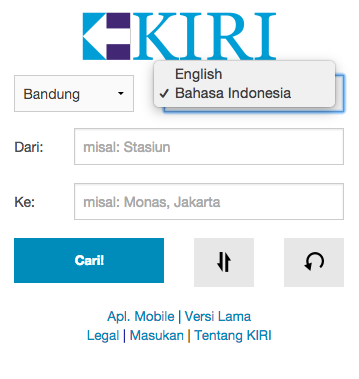
\includegraphics[scale=0.5]{Gambar/KIRI-drop-bahasa}
	\caption{Dropdown Menu Bahasa pada KIRI} 
	\label{fig:3_KIRI_drop_bahasa}
\end{figure}

Untuk menampilkan pilihan bahasa, menggunakan \textit{tag} HTML \verb!option!. Pada bagian ini, hanya cek jika sudah dilakukan lokalisasi ke Bahasa Indonesia, maka opsi yang terpilih adalah Bahasa Indonesia. Kode dapat dilihat pada \ref{lst_3_php_dropdown_bahasa_tampilan}

\begin{lstlisting}[caption=Menampilkan pilihan bahasa kepada pengguna ,label = {lst_3_php_dropdown_bahasa_tampilan}]
..
<select class="fullwidth" id="localeselect">
	<option value="en">English</option>
	<option value="id"
		<?php if ($locale == $proto_locale_indonesia) print " selected"; ?>>Bahasa
		Indonesia</option>
</select>
..
\end{lstlisting}

Ketika memilih \textit{dropdown} bahasa, memanggil \textit{method} JavaScript dengan \textit{parameter} berupa fungsi yang berisi menambahkan URL dengan \textit{query} \verb!locale=id! atau \verb!locale=en!. Kode dapat dilihat pada kode listing \ref{lst_3_php_dropdown_bahasa_fungsi}.

\begin{lstlisting}[caption=Fungsi JavaScript untuk Internationalization ,label = {lst_3_php_dropdown_bahasa_fungsi}]
..
// Event handlers
var localeSelect = $('#localeselect');
localeSelect.change(function() {
	// IE fix: when window.location.origin is not available 
	if (!window.location.origin) {
		window.location.origin = window.location.protocol + "//" + window.location.hostname + (window.location.port ? ':' + window.location.port: '');
	}
	window.location.replace(window.location.origin + "?locale=" + localeSelect.val());
});
..
\end{lstlisting}


\subsubsection{Textfield}
\textit{Textfield} pada KIRI menggunakan PHP agar dapat dilakukan proses Internationalization, seperti pada kode listing \ref{lst_3_php_textfield_from} untuk \textit{textfield} tempat asal dan kode listing \ref{lst_3_php_textfield_to} untuk \textit{textfield} tempat tujuan. Textfield pada KIRI dapat menerima dua masukan pengguna, yaitu:

\begin{lstlisting}[caption=Menampilkan \textit{textfield} tempat awal kepada pengguna ,label = {lst_3_php_textfield_from}]
..
<div class="small-2 columns">
	<label for="startInput" class="inline"><?php print $index_from; ?></label>
</div>
<div class="small-10 columns">
	<input type="text" id="startInput" value=""
		placeholder="<?php print $index_placeholder_start; ?>">
</div>
..
\end{lstlisting}

\begin{lstlisting}[caption=Menampilkan \textit{textfield} tempat tujuan kepada pengguna ,label = {lst_3_php_textfield_to}]
..
<div class="small-2 columns">
	<label for="finishInput" class="inline"><?php print $index_to; ?></label>
</div>
<div class="small-10 columns">
	<input type="text" id="finishInput" value=""
		placeholder="<?php print $index_placeholder_finish; ?>">
</div>
..
\end{lstlisting}

\begin{enumerate}
	\item \textbf{Textfield dengan Masukan Nama Tempat}, pengguna dapat memasukkan nama tempat asal dan tujuan (Gambar \ref{fig:3_KIRI_textfield_nama})
	
	\begin{figure}[H]
		\centering
		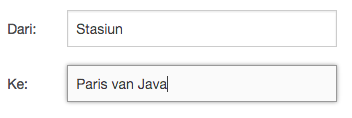
\includegraphics[scale=0.5]{Gambar/KIRI-textfield-nama}
		\caption{Input User(Nama Tempat)} 
		\label{fig:3_KIRI_textfield_nama}
	\end{figure}
	
	\item \textbf{Textfield dengan Masukan Klik Peta}, pengguna memasukkan koordinat tempat asal dan tujuan dengan klik pada peta. Dengan melakukan klik pada peta, textfield tempat asal dan tujuan akan akan secara otomatis terisi oleh koordinat masing-masing tempat (Gambar \ref{fig:3_KIRI_textfield_koord}).
	
	\begin{figure}[H]
		\centering
		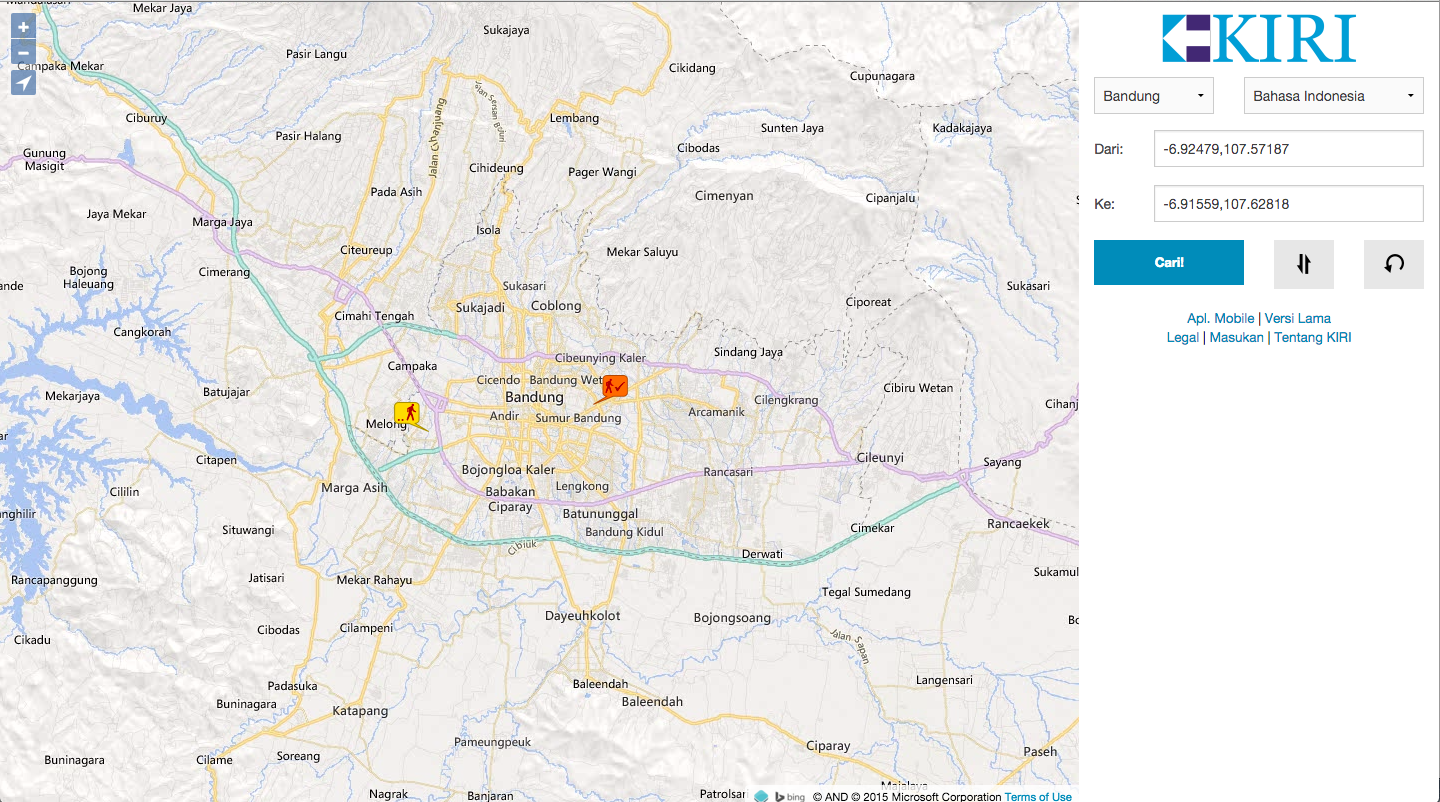
\includegraphics[scale=0.3]{Gambar/KIRI-textfield-koord}
		\caption{Input User(Klik pada peta)} 
		\label{fig:3_KIRI_textfield_koord}
	\end{figure}
	
	Agar peta dapat diklik, maka memanggil method \verb!on! dengan parameter `click` dan fungsi yang akan diimplementasikan ketika melakukan klik pada peta. Isi fungsi tersebut adalah pertama melakukan pengecekan apabila textfield tempat asal atau tempat tujuan kosong, maka membuat geometry yang merupakan objeck ol.geom.Point dengan parameter koordinat pada peta yang diklik oleh pengguna, lalu membuat marker dengan gambar start.png bila textfield tempat asal kosong atau finish.png bila textfield tempat tujuan kosong. Setelah itu, menambahkan fitur marker ke inputVectorSource yang akan ditampilkan pada peta dan menulis koordinat pada textfield tempat asal atau tempat tujuan. Kode dapat dilihat pada kode listing \ref{lst_3_php_textfield_koord_kode}.
	
	\begin{lstlisting}[caption=Membuat \textit{event} klik pada peta,label = {lst_3_php_textfield_koord_kode}]
..
// Map click event
map.on('click', function(event) {
    	if ($('#startInput').val() === '') {
		markers['start'] = new ol.Feature({
			geometry: new ol.geom.Point(event.coordinate)
		})
		markers['start'].setStyle(new ol.style.Style({
			image: new ol.style.Icon({
				src: 'images/start.png',
				anchor: [1.0, 1.0]
			})
		}));
		inputVectorSource.addFeature(markers['start']);
    		$('#startInput').val(latLngToString(ol.proj.transform(event.coordinate, 'EPSG:3857', 'EPSG:4326')));
    	} else if ($('#finishInput').val() === '') {
		markers['finish'] = new ol.Feature({
			geometry: new ol.geom.Point(event.coordinate)
		})
		markers['finish'].setStyle(new ol.style.Style({
			image: new ol.style.Icon({
				src: 'images/finish.png',
				anchor: [0.0, 1.0]
			})
		}));
		inputVectorSource.addFeature(markers['finish']);
    		$('#finishInput').val(latLngToString(ol.proj.transform(event.coordinate, 'EPSG:3857', 'EPSG:4326')));
    	}
});
..
\end{lstlisting}

\end{enumerate}

\subsubsection{Tombol Swap}
Pengguna dapat menukar isi dari \textit{textfield} tempat asal dan tujuan. Pertama kali yang dilakukan adalah mencari pada dokumen dengan \textit{id} swapbutton dan memanggil \textit{method} \verb!click! dengan \textit{parameter} fungsi swapInput seperti pada kode listing \ref{lst_3_php_swap}. Fungsi swapInput berisi melakukan pencarian pada dokumen dengan id startInput dan finishInput. Melakukan penampungan sementara dengan mengambil isi dari textfield tempat asal, lalu mengubah isi dari textfield tempat asal dengan tujuan dan mengubah isi dari textfield tempat tujuan dengan isi dari penampungan sementara. Setelah itu, jika kedua textfield ada isinya, melakukan pencarian rute. Kode dapat diliihat pada kode listing \ref{lst_3_php_swap_fungsi}.

\begin{lstlisting}[caption=\textit{Method} untuk memanggil fungsi JavaScript ketika tombol \textit{swap} ditekan ,label = {lst_3_php_swap}]
..
$('#swapbutton').click(swapInput);
..
\end{lstlisting}

\begin{lstlisting}[caption=Fungsi JavaScript untuk menukar isi \textit{textfield} tempat asal dan tujuan ,label = {lst_3_php_swap_fungsi}]	
/**
 * Swap the inputs
 */
function swapInput() {
	var startInput = $('#startInput');
	var finishInput = $('#finishInput');
	var temp = startInput.val();
	startInput.val(finishInput.val());
	finishInput.val(temp);
	coordinates['start'] = null;
	coordinates['finish'] = null;
	if (startInput.val() != '' && finishInput.val() != '') {
		findRouteClicked();
	}
}
\end{lstlisting}

\subsubsection{Tombol Reset}
Pengguna dapat melakukan pemilihan tempat dari awal dan mengulang tampilan peta. Pertama kali yang dilakukan adalah mencari pada dokumen dengan \textit{id} resetbutton dan memanggil \textit{method} \verb!click! dengan \textit{parameter} fungsi resetScreen seperti pada kode listing \ref{lst_3_php_reset}. 

\begin{lstlisting}[caption=\textit{Method} untuk memanggil fungsi JavaScript ketika tombol \textit{reset} ditekan ,label = {lst_3_php_reset}]
..
$('#resetbutton').click(resetScreen);
..
\end{lstlisting}

Fungsi resetScreen berisi berbagai fungsi seperti pada kode listing \ref{lst_3_php_reset_fungsi}, yaitu:

\begin{lstlisting}[caption=Fungsi JavaScript resetScreen ,label = {lst_3_php_reset_fungsi}]	
function resetScreen() {
	clearRoutingResultsOnTable();
	clearRoutingResultsOnMap();
	clearAlerts();
	clearStartFinishMarker();
	$.each(['start', 'finish'], function(sfIndex, sfValue) {
		var placeInput = $('#' + sfValue + 'Input');
		placeInput.val('');	
		placeInput.prop('disabled', false);
		$('#' + sfValue + 'Select').addClass('hidden');
	});
}
\end{lstlisting}

\begin{enumerate}
	\item \textbf{Fungsi clearRoutingResultsOnMap}\\
	Fungsi untuk menghapus pada resultVectorSource yang merupakan berbagai \textit{marker} pada peta sebagai hasil pencarian rute dan memperbarui peta. Kode dapat dilihat pada kode listing \ref{lst_3_php_reset_clearMap}.
	\begin{lstlisting}[caption=Fungsi JavaScript untuk menghapus hasil pencarian rute pada peta ,label = {lst_3_php_reset_clearMap}]
	function clearRoutingResultsOnMap() {
		resultVectorSource.clear();
		updateRegion(region, false);
	}
	\end{lstlisting}
	
	\item \textbf{Fungsi clearRoutingResultsOnTable}\\
	Fungsi untuk menghapus tampilan tabel sebagai hasil pencarian rute yang akan ditampilkan pada pengguna. Kode dapat dilihat pada kode listing \ref{lst_3_php_reset_clearTable}.
	
	\begin{lstlisting}[caption=Fungsi JavaScript untuk menghapus tampilan tabel,label = {lst_3_php_reset_clearTable}]
	function clearRoutingResultsOnTable() {
		$('.tabs').remove();
		$('.tabs-content').remove();
	}
	\end{lstlisting}
	
	\item \textbf{Fungsi clearAlerts}\\
	Fungsi untuk menghapus \textit{alerts} sebagai tanda yang akan ditampilkan kepada pengguna, seperti sedang melakukan pencarian rute atau masalah koneksi. Kode dapat dilihat pada kode listing \ref{lst_3_php_reset_clearAlerts}.
	
	\begin{lstlisting}[caption=Fungsi JavaScript untuk menghilangkan \textit{alerts},label = {lst_3_php_reset_clearAlerts}]
	function clearAlerts() {
		$('.alert-box').remove();
	}
	\end{lstlisting}
	
	\item \textbf{Fungsi clearRoutingResultsOnMap}\\
	Fungsi untuk menghapus \textit{markers} tempat awal dan tujuan, lalu menghapus fitur pada inputVectorSource. Kode dapat dilihat pada kode listing \ref{lst_3_php_reset_clearMarker}.
	
	\begin{lstlisting}[caption=Fungsi JavaScript untuk menghilangkan \textit{alerts},label = {lst_3_php_reset_clearMarker}]
	function clearStartFinishMarker() {
		if (markers['start'] != null) {
			markers['start'] = null;
		}
		if (markers['finish'] != null) {
			markers['finish'] = null;
		}
		inputVectorSource.clear();
	}
	\end{lstlisting}
	
\end{enumerate}

\subsubsection{Tombol Find}
Pengguna dapat mencari rute untuk sampai ke tujuan (Gambar \ref{fig:3_KIRI_find}). Pengguna dapat memilih rute alternatif yang sudah disediakan KIRI jika ada (Gambar \ref{fig:3_KIRI_find_alternate}).

\begin{figure}[H]
	\centering
	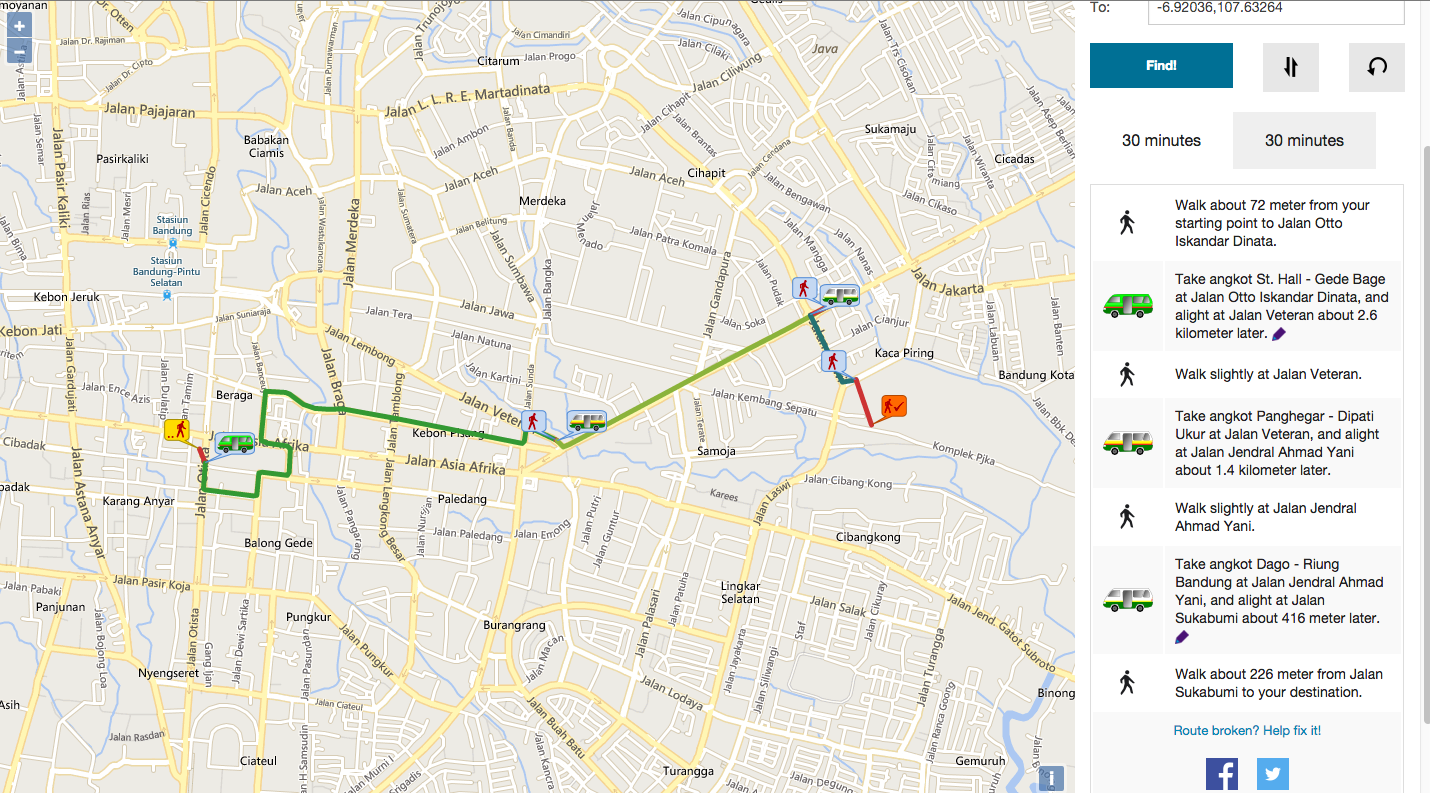
\includegraphics[scale=0.3]{Gambar/KIRI-find}
	\caption{Contoh Pencarian Rute pada KIRI} 
	\label{fig:3_KIRI_find}
\end{figure}

\begin{figure}[H]
	\centering
	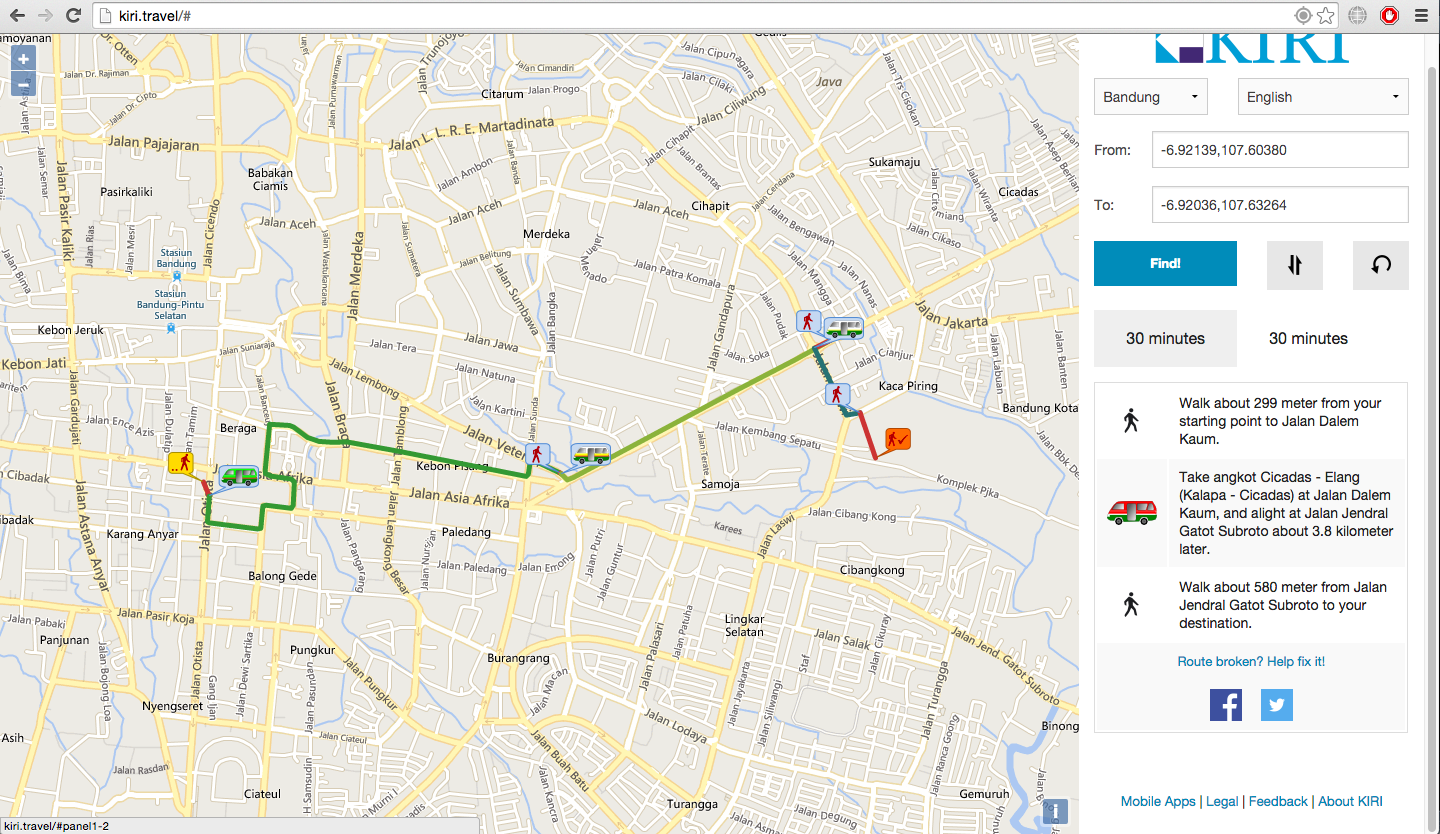
\includegraphics[scale=0.3]{Gambar/KIRI-find-alternate}
	\caption{Contoh Rute Alternatif pada KIRI} 
	\label{fig:3_KIRI_find_alternate}
\end{figure}

Hal yang pertama kali dilakukan adalah melakukan validasi jika salah satu textfield kosong, maka akan langsung membatalkan proses dan memberi alert kepada pengguna. Jika tidak kosong, maka akan memunculkan alert `mohon menunggu`. 
Setelah itu melakukan pengecekan apakah isi dari textfield merupakan format yang bener untuk garis lintang dan bujur. Jika formatnya benar, maka dimasukkan ke dalam array coordinates dan melakukan penambahan completedLatLon yang berfungsi untuk mengetahui apakah kedua textfield sudah benar formatnya untuk dilakukan pencarian rute. Jika formatnya tidak benar, maka melakukan pengecekan array coordinates kosong atau tidak. 
Jika kosong, maka melakukan pencarian pilihan tempat yang akan menjadi tempat sugesti yang diberikan kepada pengguna. Jika tidak kosong, maka memanggil fungsi checkCoordinatesThenRoute dengan parameter berupa coordinates. Terakhir, melakukan pengecekan completedLatLon jika isinya sama dengan dua, maka memanggil fungsi checkCoordinatesThenRoute. Kode dapat dilihat pada kode listing \ref{lst_3_php_find_fungsi}.

\begin{lstlisting}[caption=Fungsi JavaScript untuk ketika tombol \textit{find} ditekan,label = {lst_3_php_find_fungsi}]
/**
 * A function that will be called when find route button is clicked
 * (or triggered by another means)
 */
function findRouteClicked() {
	// Validate
	var cancel = false;
	$.each(['start', 'finish'], function(sfIndex, sfValue) {
		if ($('#' + sfValue + 'Input').val() === '') {
			cancel = true;		
			return;
		}
	});
	if (cancel) {
		showAlert(messageFillBoth, 'alert');			
		return;
	}
	
	clearAlerts();
	clearRoutingResultsOnTable();
	showAlert(messagePleaseWait, 'secondary');
	
	var completedLatLon = 0;
	$.each(['start', 'finish'], function(sfIndex, sfValue) {
		var placeInput = $('#' + sfValue + 'Input');
		var placeSelect = $('#' + sfValue + 'Select');
		if (isLatLng(placeInput.val())) {
			coordinates[sfValue] = placeInput.val();
			completedLatLon++;
		} else {
			if (coordinates[sfValue] == null) {
				// Coordinates not yet ready, we do a search place
				protocol.searchPlace(
						placeInput.val(),
						region,
						function(result) {
							placeSelect.empty();
							placeSelect.addClass('hidden');
							if (result.status != 'error') {
								if (result.searchresult.length > 0) {
									$.each(result.searchresult, function(index, value) {
										var placeSelect = $('#' + sfValue + 'Select');
										placeSelect
									         .append($('<option></option>')
									         .attr('value',value['location'])
									         .text(value['placename']));
										placeSelect.removeClass('hidden');
									});
									coordinates[sfValue] = result.searchresult[0]['location'];
									checkCoordinatesThenRoute(coordinates);
								} else {
									clearSecondaryAlerts();
									clearRoutingResultsOnMap();
									showAlert(placeInput.val() + messageNotFound, 'alert');
								}
							} else {
								clearSecondaryAlerts();
								clearRoutingResultsOnMap();
								showAlert(messageConnectionError, 'alert');
							}
						});
			} else {
				// Coordinates are already available, skip searching
				checkCoordinatesThenRoute(coordinates);
			}
		}
	});
	if (completedLatLon == 2) {
		checkCoordinatesThenRoute(coordinates);
	}
}
\end{lstlisting}

Fungsi checkCoordinatesThenRoute melakukan pengecekan jika array coordinates tempat awal dan tempat tujuan tidak kosong maka melakukan protocol.findRoute. Jika hasil results sama dengan `ok`, maka menunjukkan rute pencarian. Jika hasil result bukan `ok`, maka akan menampilkan alert `gangguan koneksi`. Kode dapat dilihat pada kode listing \ref{lst_3_php_find_checkRoute}.
\begin{lstlisting}[caption=Fungsi JavaScript checkCoordinatesThenRoute,label = {lst_3_php_find_checkRoute}]
/**
 * Check if coordinates are complete. If yes, then start routing.
 * @param coordinates the coordinates to check.
 */
function checkCoordinatesThenRoute(coordinates) {
	if (coordinates['start'] != null && coordinates['finish'] != null) {
		protocol.findRoute(
				coordinates['start'],
				coordinates['finish'],
				locale,
				function(results) {
					if (results.status === 'ok') {
						showRoutingResults(results);
					} else {
						clearSecondaryAlerts();
						showAlert(messageConnectionError, 'alert');
					}
				});
	}
}
\end{lstlisting}

\subsection{Internationalization}
Penggunaan Internationalization (i18n) pada PHP dengan cara deklarasi semua variabel yang akan digunakan pada proses i18n terlebih dahulu, misalnya buat file dengan nama tirtayasa\_en.php untuk Bahasa Inggris dan tirtayasa\_id.php untuk Bahasa Indonesia. Pada setiap file tersebut, masukkan \textit{script} PHP untuk menentukan teks yang keluar pada halaman \textit{web} seperti pada kode listing \ref{lst_3_i18n_en} dan kode listing \ref{lst_3_i18n_id}. 

\begin{lstlisting}[caption=Script PHP untuk Bahasa Inggris,label = {lst_3_i18n_en}]
<?php

	$index_about_kiri = "About KIRI";
	$index_apps = "Mobile Apps";
	$index_advanced_ = "Advanced...";
	$index_buyticket = "BUY TICKET";
	$index_connectionerror = 'Connection problem';
?>
\end{lstlisting}


\begin{lstlisting}[caption=Script PHP untuk Bahasa Indonesia,label = {lst_3_i18n_id}]
<?php
	$index_about_kiri = "Tentang KIRI";
	$index_apps = "Apl. Mobile";
	$index_advanced_ = "Lanjut...";
	$index_buyticket = "BUY TICKET";
	$index_connectionerror = 'Gangguan koneksi';
?>
\end{lstlisting}

Setelah itu, masukkan \textit{script} PHP pada \textit{tag} HTML yang ingin diubah saat dilakukan i18n. Adanya \textit{script} PHP pada tag HTML, maka teks akan berubah jika dilakukan i18n seperti pada kode listing \ref{lst_3_i18n_php}.

\begin{lstlisting}[caption=Script PHP untuk Internationalization,label = {lst_3_i18n_php}]
	...
	<label for="startInput" class="inline"><?php print $index_from; ?></label>
	<label for="finishInput" class="inline"><?php print $index_to; ?></label>
	<a href="#" class="small button expand" id="findbutton"><strong><?php print $index_find; ?></strong></a>
	...
\end{lstlisting}

\subsection{Pencarian Rute}
Pencarian rute pada KIRI dilakukan di \textit{server side}, yaitu pada \textit{file} handle.php. Langkah awal pada ``handle.php'' dapat dijelaskan sebagai berikut:
\begin{enumerate}
	\item ``constants.php'' untuk menyiapkan data yang akan dipakai pada halaman \textit{web}.
	\item ``utils.php'' untuk fungsi manipulasi data, koneksi \textit{database}, mengirimkan pencatatan, dan melakukan validasi.
	\begin{itemize}
		\item Fungsi ``init\_mysql'' untuk memuat koneksi \textit{database} dengan memasukkan \textit{host, username, password}, dan \textit{database} yang digunakan pada MySQL.
		\item Fungsi ``log\_statistic'' untuk pencatatan data pada \textit{database}.
		\item Fungsi ``die\_nice'' untuk mengirimkan pesan kesalahan.
		\item Fungsi ``check\_apikey\_validity'' untuk pengecekan apikey yang digunakan ada atau tidak.
		\item Fungsi ``retrieve\_from\_post'' untuk mengambil data pada URL dengan memanggil method ``\$\_POST'' dengan parameter \textit{key} yang digunakan.
		\item Fungsi ``retrieve\_from\_get'' untuk mengambil data pada URL dengan memanggil method ``\$\_GET' dengan parameter \textit{key} yang digunakan.
		\item Fungsi ``retrieve\_from\_cache'' untuk mengambil data pada \textit{database} \textit{cache} dengan parameter `type' dan `cacheKey'.
		\item Fungsi ``put\_to\_cache'' untuk memasukkan data pada \textit{database} \textit{cache} dengan parameter `type' , `cacheKey', dan `cacheValue'.
	\end{itemize}
	\item \verb!start_working! untuk menyiapkan header pada PHP.
	\begin{itemize}
		\item Fungsi ``header('Content-Type: application/json')'' untuk menghasilkan \textit{output} JSON.
		\item Fungsi ``header('Cache-control: no-cache')'' digunakan pada HTTP/1.1 dan fungsi ``header('Pragma: no-cache')'' digunakan pada HTTP/1.0. Keduanya berfungsi untuk mencegah pengguna menyimpan \textit{cache response}.
	\end{itemize}
	\item \verb!init_mysql! untuk koneksi pada database menggunakan MySQL. 
	\item Mendapatkan data `mode', `version', dan `apikey' dari \textit{method} \verb!POST! masing-masing dengan \textit{parameter} `mode', `version', dan `apikey'.
	\item Jika data ``\texttt{version = null}'', maka isi dengan ``1''. 
	\item Melakukan pengecekan `apikey' apakah ada di \textit{database} atau tidak. Jika ada, cek lagi apakah ada pengecualian IP komputer pada database.
\end{enumerate}

\subsubsection{Mode Findroute}
Bagian ini terletak di baris 14-181 dari ``handle.php'' (kode \ref{lst:handle.php}). Langkah pertama yang dilakukan adalah memasukkan data `start', `finish', dan `locale' dengan mendapatkan \textit{method} \verb!POST! masing-masing dengan \textit{parameter} `start', `finish', dan `locale'. Tetapi sebelum dimasukkan, memanggil \textit{method} \verb!addslashes! yang berfungsi jika ada karakter spesial seperti ' atau " tidak dianggap sebagai suatu String yang berbeda. Setelah itu melakukan pengecekan untuk lokalisasi. Jika ada, load file (lokalisasi Bahasa Inggris atau lokalisasi Bahasa Indonesia). Setelah itu melakukan pengecekan variabel `presentation', ada dua yaitu  \textit{mobile} atau \textit{desktop}. Melakukan pengecekan version yang digunakan:
\begin{itemize}
	\item Jika ``\texttt{version >= 2}'', maka memasukkan data `count' dengan ``1''. Jika ``\texttt{presentation = mobile}'', maka memasukkan data `count' dengan jumlah \textit{array alternatives}. Setelah itu melakukan pengulangan sebanyak `count' yang berisi:\\
		Menambahkan \textit{query URL} menjangan dengan:
		\begin{itemize}
			\item 	``?start=koordinat start'' dan ``finish=koordinat finish''.
			\item `mw', `wm', dan `pt' masing-masing dengan nilai dari \textit{array alternative} satu persatu dengan indeks `mw', `wm', dan `pt'.
			\item memanggil fungsi file\_get\_content yang akan mengembalikan ``FALSE'' jika gagal dan mengembalikan JSON pesan kesalahan. Jika berhasil akan mendapatkan String dengan \textit{URL} dari menjangan, pembacaan maksimal sebanyak 51200 \textit{bytes}.
			\item memasukkan ke \textit{array} `results' yang mempunyai indeks `result' dengan nilai ``true''.
		\end{itemize}
	\item Jika ``\texttt{version < 2}'', langsung akses \textit{URL} menjangan dengan \textit{query} ``?start=koordinat start'' dan ``finish=koordinat finish''.
\end{itemize}

Langkah selanjutnya adalah pengulangan sejumlah data `results' menjadi `result' dengan nilai yang dimasukkan ke data `dummy' yang berisi:
\begin{itemize}
	\item Membuat data `steps' yang berisi data `result' yang telah dipisahkan per baris.
	\item Melakukan pengulangan setiap data `steps' dan dimasukkan ke `step' yang berisi:
	\begin{itemize}
		\item Membuang spasi yang ada pada data `step'. Jika `step' sudah tidak ada isinya, melanjutkan ke langkah selanjutnya.
		\item Jika ``\texttt{step = none}'', melakukan pengecekan pada banyaknya data `results'. Jika banyak data `results' bukan satu berarti ada rute alternatif dan akan melanjutkan ke langkah selanjutnya. Tetapi jika banyak data `results' satu, tidak ada rute alternatif.
		\item Mendaftarkan data `means', `means\_detail', `route', `distance', dan `nearbyplaceids' yang didapat dari data `step' yang telah dipisahkan ``/''. Jika salah satu data kosong, akan menutup koneksi SQL dan mengeluarkan pesan kesalahan.
		\item Inisialisasi data `points' yang didapat dari data `route' yang sudah dipisahkan spasi, inisialisasi data `from' dari data `points' dengan indeks 0 dan inisialisasi data `to' dari data `points' dengan indeks terakhir.
		\item Jika nilai data `points' ada yang sama dengan ``start'', maka mengganti data `points' tersebut dengan data `start'. Jika nilai data `points' ada yang sama dengan ``finish'', maka mengganti data `points' tersebut dengan data `finish'.
		 \item Memasukkan data `humanized\_from' dengan memanggil fungsi humanize\_point dengan \textit{parameter} `from' dan `humanized\_to' dengan memanggil fungsi humanize\_point dengan \textit{parameter} `to'.
		 \item Jika ``\texttt{means = walk}'', melakukan pengecekan ``\texttt{humanized\_from = humanized\_to}''. Jika ``\texttt{presentation != mobile}'', maka memasukkan `message\_walk\_samestreet' ke variabel `humanreadable'. Mengganti ``\%from'' yang ada di `humanreadable' dengan value ``humanized\_from'', mengganti ``\%distance'' yang ada di `humanreadable' dengan value ``distance'' yang dipresentasikan sesuai format wilayah pengguna. Lalu menghitung waktu tempuh yg dibutuhkan.
		 \item Jika ``\texttt{means != walk}'', melakukan pencarian pada \textit{database} `tracks' digabung dengan `tracktypes' dengan kolom nama jalur, tipe jalur yang digunakan, \textit{URL} untuk melakukan pemesanan (jika XTrans), kecepatan transportasi, dan informasi internal jalur dimana ``\texttt{trackTypeId = means}'' pada tabel `tracktypes' dan `tracks' serta ``\texttt{trackid = means\_detail}'' pada tabel `tracks'. Jika ada hasil dari pencarian \textit{database}, memasukkan hasil dengan indeks ke-nol ke `readable\_track\_name' dan memasukkan hasil dengan indeks pertama ke `track\_type\_name'. Jika ``\texttt{presentation = mobile}'', menambahkan data `humanized\_from' dengan ``\%fromicon'' dan `humanized\_to' dengan  ``\%toicon''. Memasukkan `message\_angkot' ke data `humanreadable'. Memperbarui  `humanreadable' dengan mengganti ``\%from'' yang ada di `humanreadable' dengan value ``humanized\_from'', memperbarui `humanreadable' dengan mengganti ``\%to'' yang ada di `humanreadable' dengan value ``humanized\_to'', memperbarui `humanreadable' dengan mengganti  ``\%distance'' yang ada di `humanreadable' dengan value ``distance'' yang dipresentasikan sesuai format wilayah pengguna, memperbarui `humanreadable' dengan mengganti ``\%trackname'' yang ada di `humanreadable' dengan value `readable\_track\_name', dan memperbarui `humanreadable' dengan mengganti ``\%tracktype'' yang ada di `humanreadable' dengan value `track\_type\_name'. Membuat `speed' dengan mengambil hasil pencarian dari indeks ke-empat yang sudah dijadikan Integer, lalu menghitung waktu tempuh. Melakukan pengecekan `URL jalur' dan `extraParameter' kosong tidak. Jika tidak kosong maka menambahkan data `booking\_url' dengan menambahkan nilai `URL jalur' dan `extraParameter'. Lalu melakukan pengecekan hasil pencarian `internalinfo' dimulai dengan string ``angkotwebid:''. Jika dimulai dengan ``angkotwebid:'', maka mendapatkan \textit{array} `token' dengan memisahkan ``:'' pada `internalInfo'. Membuat `editor\_url' didapat dari awalan \textit{URL} angkotwebid, token dengan indeks pertama + akhiran \textit{URL} angkotwebid. 
		 \item Jika ``\texttt{humanreadable != null}'', memasukkan `route\_output' dengan isi array dari `means', `means\_detail', `points', `humanreadable', `booking\_url', dan `editor\_url'. 
	\end{itemize}
	\item Memasukkan routing\_result dengan indeks `steps' dengan nilai `route\_output'
	\item Memasukkan routing\_result dengan indeks `traveltime' dengan nilai jam dan menit dari  `travel\_time'.
	\item Memasukkan kembali `routing\_result'.
\end{itemize}
Setelah itu, membuat pencatatan statistik sesuai dengan `apikey' yang digunakan dan menutup koneksi ke \textit{database}. Jika ``\texttt{version != null}'' dan ``\texttt{version >= 2}'', maka print String yang sudah di \textit{encode} menjadi JSON dengan ``status : ok'', ``routingresult : hasil pencarian rute''. Jika ``\texttt{version = null}'' dan ``\texttt{version < 2}'', maka print String yang sudah di \textit{encode} menjadi JSON dengan ``status : ok'', ``routingresult : langkah-langkah hasil pencarian rute'', dan ``traveltime : waktu tempuh''.

\subsubsection{Mode Search}
Bagian ini terletak di baris 183-280 dari ``handle.php'' (kode \ref{lst:handle.php}). Langkah pertama yang dilakukan adalah memasukkan data `querystring', `apikey', dan `region' dengan mendapatkan \textit{method} \verb!POST! masing-masing dengan \textit{parameter} `querystring', `apikey', dan `region'. Jika ``\texttt{region = null}'', maka isi `region' dengan ``bandung''. Melakukan pengulangan sejumlah data `regioninfos' dengan nilai yang dimasukkan ke data `value' yang berisi:
\begin{itemize}
	\item Mencari dalam `querystring' ada \textit{pattern} ``/searchplace/i'', dimana `searchplace' diambil dari `value' dengan indeks `searchplace\_regex' dan tampilkan pada \textit{array} `matches'. Jika terdapat pattern tersebut, maka memasukkan `region' dengan `key', memperbarui `querystring' dengan mengambil panjang kalimat sebanyak `matches' dengan indeks nol dan pertama dari `querystring', dan memberhentikan pengulangan.
	\item Mengubah `querystring' menjadi format \textit{URL}.
	\item Memasukkan `cached\_searchplace' dengan mengambil \textit{cache} dengan tipe ``searchplace'' dan \textit{key} `region'/`querystring'. Jika ``\texttt{cached\_searchplace != null}'', maka membuat JSON untuk \textit{output} dengan ``status : ok'', ``searchresult : mengubah JSON menjadi String dari cached\_searchplace ``,``attributions : null''. \\
	Jika ``\texttt{cached\_searchplace = null}'', memasukkan data `lat', `lon', dan `radius' yang didapat dari `regioninfos' dengan indeks `region' dengan \textit{key}`lat', `lon', dan `radius'. Memasukkan `result' dengan hasil akses \textit{URL} dari data `full\_url'. Jika ``\texttt{result = FALSE}'' atau jumlah ``\texttt{result > maximum\_http\_response\_size}'', maka mengeluarkan pesan kesalahan. Setelah itu, memasukkan `json\_result' dengan mengubah JSON menjadi String dari data `result'. Jika `json\_result' dengan indeks status adalah ``OK'' atau ``ZERO\_RESULTS'', maka menyiapkan array `search\_result'. Jika hasilnya ``ZERO\_RESULTS'', maka mengeluarkan catatan kesalahan dan memperbarui data `size' menjadi ``0''. Jika hasilnya ``OK'', maka mengambil angka minimal antara `result' dan `search\_maxresult'. Melakukan pengulangan dari nol sampai dengan `size' yang dinisialkan dengan `i':
	\begin{itemize}
		\item Memasukkan data `current\_venue' dengan `json\_result' indeks results dengan key `i'.
		\item Memasukkan data `search\_result' dengan indeks `i' dan key `placename' yang isinya adalah `current\_venue' dengan indeks name.
		\item Memasukkan data `search\_result' dengan indeks `i' dan key `location' yang isinya adalah String yang sudah diformat ``\%.latlonlf\%.latlonlf'' yang nilainya diambil dari `current\_venue' dengan indeks geometry dan location dengan key lat dan lng.
		\item Menyiapkan `json\_output' yang merupakan array dari ``status : ok'', ``searchresult : search\_result'' yang merupakan hasil pencarian rute, dan ``attributions : null''.
		\item Mengirim catatan dengan `apikey' yang digunakan
		\item Memasukkan ke \textit{cache} dengan tipe `cache\_searchplace', \textit{key} ``region/querystring'' yang berisi JSON `search\_result'.
	\end{itemize}
	\item Mengeluarkan hasil JSON `json\_output'.
\end{itemize}

\subsubsection{Mode Reporterror}
Bagian ini terletak di baris 282-284 dari ``handle.php'' (kode \ref{lst:handle.php}). Langkah pertama yang dilakukan adalah mendapatkan `errorcode' dari \textit{method} \verb!POST! dengan \textit{parameter} ``errorcode''. Mencatat kesalahan dan dimasukkan ke dalam \textit{file}. Mengeluarkan JSON dengan ``status : OK'' dan memberhentikan eksekusi program.

\subsubsection{Mode Nearbytransport}
Bagian ini terletak di baris 286-313 dari ``handle.php'' (kode \ref{lst:handle.php}). Langkah pertama yang dilakukan adalah mendapatkan `start' dari \textit{method} \verb!POST! dengan \textit{parameter} ``routestart''. Jika ``\texttt{version >= 2}'', maka membuat data `lines' dengan mendapatkan String dari `menjangan\_url' + /?start=`start`. Setelah mendapatkan String tersebut, lakukan pemisahan baris. Melakukan pengulangan sebanyak `lines' yang berisi:
\begin{itemize}
	\item Melakukan pemisahan dari ``\'' dari `line', lalu mendaftarkan menjadi  `tracktypeid', `trackid',dan `distance'.
	\item Membuat data `result' dengan melakukan perintah SQL, yaitu mendapatkan `trackname' dari tabel `tracks' dimana` trackid' dan `tracktypeid` sesuai dengan yang sudah didaftarkan.
	\item Membuat data `row' dengan mengambil hasil dari data `result' dan melakukan pengulangan yang berisi:
	\begin{itemize}
		\item Membuat data `trackName' dengan mengambil `row' indeks nol.
		\item Membuat data `nearby\_result' yang merupakan array dari `trackTypeId', `trackId', `trackName', dan `distance'.
	\end{itemize}
	\item Menyortir array `nearby\_result' berdasarkan fungsi ``nearby\_result\_compare''. Fungsi ``nearby\_result\_compare'' membandingkan jarak yang diambil dari \textit{array}.
	\item Membuat catatan dengan `apikey' yang digunakan.
	\item Menyiapkan dan mengeluarkan`json\_output` dengan isi ``status : ok'', ``nearbytransports : nearby\_result''.
	
\end{itemize}

\subsubsection{Fungsi humanize\_point}
Tujuan dari fungsi ini adalah merubah lokasi dalam bentuk \textit{point} menjadi nama lokasi tempat dari \textit{point} tersebut. Fungsi ini menerima parameter `location' yang merupakan String. Fungsi ini berisi sebagai berikut:
\begin{itemize}
	\item Melakukan deklarasi variabel global untuk digunakan.
	\item Melakukan pengecekan data `location'. Jika ``\texttt{location = start}'' maka mengembalikan `message\_start'. Jika ``\texttt{location = finish}'', maka mengembalikan `message\_finish'.
	\item Jika bukan keduanya, maka memanggil fungsi ``mysqli\_escape\_string''.
	\item Melakukan pengecekan \textit{cache} ada atau tidak dengan \textit{key} `cache\_geocoding' dan bernilai sesuai dengan parameter `location' atau tidak dan dimasukkan ke data `cached\_geocode'. Jika ada nilainya, langsung mengembalikan nilai tersebut.
	\item Jika tidak ada, maka akan menambahkan \textit{query} pada \textit{URL} Google. Jika berhasil akses dan mendapatkan ``\texttt{status = OK}'', maka akan menambahkan lokasi sugesti pada pengguna. Jika ``\texttt{status != OK}'', maka akan menampilkan pesan kesalahan. 
\end{itemize}
\section{Analisis Sistem Usulan}
\label{sec:perubahan}

\subsection{Form Samping}
\subsubsection{Dropdown Menu Kota}
Untuk menampilkan pilihan kota pada \play, menampilkan semua pilihan kota yang terdapat pada KIRI. Kode dapat dilihat pada kode listing \ref{lst_3_play_dropdown_kota_tampilan}

\begin{lstlisting}[caption=Menampilkan pilihan kota kepada pengguna ,label = {lst_3_play_dropdown_kota_tampilan}]
..
<select class="fullwidth" id="regionselect">
    <option value="bdg">Bandung</option>
    <option value="jkt">Jakarta</option>
    <option value="sby">Surabaya</option>
    <option value="mlg">Malang</option>
</select>
..
\end{lstlisting}

Untuk memperbarui peta menggunakan \play, membuat fungsi JavaScript updateMap dengan parameter array Float sebagai garis bujur dan garis lintang dan zoom sebagai tingkat zoom pada peta. Kode dapat dilihat pada kode listing \ref{lst_3_play_dropdown_kota_updateMap}.

\begin{lstlisting}[caption=Fungsi JavaScript untuk memperbarui peta ,label = {lst_3_play_dropdown_kota_updateMap}]
var updateMap = function(arrLonLat,zoom){

    map.getView().setCenter(ol.proj.transform(arrLonLat, 'EPSG:4326', 'EPSG:3857'));
    map.getView().setZoom(zoom);
};
\end{lstlisting}

Untuk menambahkan aksi ketika memilih opsi \textit{dropdown} kota, pertama melakukan pencarian pada dokumen dengan \textit{id} regionselect. Handler tersebut berfungsi ketika mengganti pilihan pada dropdown, memasukkan koordinat yang tepat untuk opsi kota dan memanggil fungsi updateMap untuk memperbarui peta. Kode dapat dilihat pada kode listing \ref{lst_3_play_dropdown_kota_update}.

\begin{lstlisting}[caption=Fungsi JavaScript untuk menambahkan \textit{handler} ketika mengganti \textit{dropdown} kota ,label = {lst_3_play_dropdown_kota_update}]
var regionSelect = document.getElementById("regionselect");

var handlerRegion = function () {
    var regionValue = regionSelect.value;
    if(regionValue=="bdg")
    {
        arrLonLat = [107.60981,-6.91474];
        updateMap(arrLonLat,12);
    }else if(regionValue=="jkt")
    {
        arrLonLat = [106.84517,-6.21154];
        updateMap(arrLonLat,11);
    }else if(regionValue=="sby")
    {
        arrLonLat = [112.71908,-7.27421];
        updateMap(arrLonLat,12);
    }else
    {
        arrLonLat = [112.6319264,-7.9812985];
        updateMap(arrLonLat,13);

    }

};
regionSelect.addEventListener("change",handlerRegion,false);
\end{lstlisting}

\subsubsection{Dropdown Menu Bahasa}
Untuk menampilkan pilihan bahasa, menggunakan \textit{tag} HTML \verb!option!. Pada bagian ini. Kode dapat dilihat pada \ref{lst_3_pplay_dropdown_bahasa_tampilan}

\begin{lstlisting}[caption=Menampilkan pilihan bahasa kepada pengguna ,label = {lst_3_play_dropdown_bahasa_tampilan}]
..
<select class="fullwidth" id="localeselect">
    <option value="en">English</option>
    <option value="id">Bahasa Indonesia</option>
</select>
..
\end{lstlisting}

Ketika memilih \textit{dropdown} bahasa, pertama melakukan pencarian pada dokumen dengan \textit{id} localeselect. Setelah itu menambahkan \textit{handler} yang berisi melakukan pengecekan isi dari \textit{dropdown} bahasa, lalu memanggil \textit{method} JavaScript \verb!window.location.replace! dengan \textit{parameter} URL baru yang sesuai dengan bahasa. Kode dapat dilihat pada kode listing \ref{lst_3_play_dropdown_bahasa_fungsi}.

\begin{lstlisting}[caption=Fungsi JavaScript untuk Internationalization ,label = {lst_3_play_dropdown_bahasa_fungsi}]
..
var localeSelect = document.getElementById("localeselect");

var handlerLocale = function(){
    var localeValue = localeSelect.value;
    if(localeValue=="en")
    {
        window.location.replace("http://localhost:9000");
    }
    else if(localeValue =="id")
    {
        window.location.replace("http://localhost:9000/id");

    }
};
localeSelect.addEventListener("change",handlerLocale,false);
..
\end{lstlisting}


\subsubsection{Textfield}
Pada \play, \textit{Textfield} pada KIRI dibuat  agar dapat dilakukan proses i18n, seperti pada kode listing \ref{lst_3_play_textfield_from} untuk \textit{textfield} tempat asal dan kode listing \ref{lst_3_play_textfield_to} untuk \textit{textfield} tempat tujuan.

\begin{lstlisting}[caption=Menampilkan \textit{textfield} tempat awal kepada pengguna ,label = {lst_3_play_textfield_from}]
..
<div class="small-2 columns">
    <label for="startInput" class="inline">@Messages.get("from")</label>
</div>
<div class="small-10 columns">
    <input type="text" id="startInput" value=""
    placeholder="@Messages.get("ph_from")">
</div>
..
\end{lstlisting}

\begin{lstlisting}[caption=Menampilkan \textit{textfield} tempat tujuan kepada pengguna ,label = {lst_3_play_textfield_to}]
..
<div class="small-2 columns">
    <label for="finishInput" class="inline">@Messages.get("to")</label>
</div>
<div class="small-10 columns">
    <input type="text" id="finishInput" value=""
    placeholder="@Messages.get("ph_to")">
</div>
..
\end{lstlisting}
	
Pada \play, hal yang diubah adalah pengambilan gambar pada folder `assets/images. Kode dapat dilihat pada kode listing \ref{lst_3_play_textfield_koord_kode}.
	
	\begin{lstlisting}[caption=Membuat \textit{event} klik pada peta,label = {lst_3_play_textfield_koord_kode}]
//for map click event
map.on('click', function(event) {
    if (startInput.value === '')
    {
        markers['start'] = new ol.Feature({
            geometry: new ol.geom.Point(event.coordinate)
        })
        markers['start'].setStyle(new ol.style.Style({
            image: new ol.style.Icon({
                src: '/assets/images/start.png',
                anchor: [1.0, 1.0]
            })
        }));
        inputVectorSource.addFeature(markers['start']);
        startInput.value = latLngToString(ol.proj.transform(event.coordinate, 'EPSG:3857', 'EPSG:4326'));
    }else if (finishInput.value === '') {
        markers['finish'] = new ol.Feature({
            geometry: new ol.geom.Point(event.coordinate)
        })
        markers['finish'].setStyle(new ol.style.Style({
            image: new ol.style.Icon({
                src: 'assets/images/finish.png',
                anchor: [0.0, 1.0]
            })
        }));
        inputVectorSource.addFeature(markers['finish']);
        finishInput.value = latLngToString(ol.proj.transform(event.coordinate, 'EPSG:3857', 'EPSG:4326'));
    }
});

\end{lstlisting}

\subsubsection{Tombol Swap}
Pengguna dapat menukar isi dari \textit{textfield} tempat asal dan tujuan. Pertama kali yang dilakukan adalah mencari pada dokumen dengan \textit{id} swapbutton dan menambahkan fungsi seperti pada kode listing \ref{lst_3_play_swap}. Fungsi tersebut berisi menukar isi dari textfield tempat asal dan tempat tujuan seperti pada kode listing \ref{lst_3_php_swap_fungsi}.

\begin{lstlisting}[caption=\textit{Method} untuk memanggil fungsi JavaScript ketika tombol \textit{swap} ditekan ,label = {lst_3_play_swap}]
..
var swapBtn = document.getElementById("swapbutton");

swapBtn.addEventListener("click",swapInput);
..
\end{lstlisting}

\begin{lstlisting}[caption=Fungsi JavaScript untuk menukar isi \textit{textfield} tempat asal dan tujuan ,label = {lst_3_pplay_swap_fungsi}]	

/**
 * Swap the inputs
 */
function swapInput() {
    var temp = startInput.value;

    startInput.value = finishInput.value;
    finishInput.value = temp;

    coordinates['start'] = null;
    coordinates['finish'] = null;
    
    if(startInput.value != "" && finishInput.value != ""){
        findRouteClicked();
    }
}
\end{lstlisting}

\subsubsection{Tombol Reset}
Pertama kali yang dilakukan adalah mencari pada dokumen dengan \textit{id} resetbutton dan menambahkan fungsi reset ketika tombol reset ditekan seperti pada kode listing \ref{lst_3_play_reset}. 

\begin{lstlisting}[caption=\textit{Method} untuk memanggil fungsi JavaScript ketika tombol \textit{reset} ditekan ,label = {lst_3_play_reset}]
..
var resetBtn = document.getElementById("resetbutton");
resetBtn.addEventListener("click",reset);
..
\end{lstlisting}

Fungsi reset berisi berbagai fungsi seperti pada kode listing \ref{lst_3_php_reset_fungsi}, yaitu:

\begin{lstlisting}[caption=Fungsi JavaScript reset ,label = {lst_3_play_reset_fungsi}]	
/**
 * Reset Screen
 */
function reset() {
    clearRoutingResultsOnTable();
    clearRoutingResultsOnMap();
    clearAlerts();
    clearStartFinishMarker();

    var x = ['start', 'finish'];
    for (x in markers, function(sfIndex, sfValue) {
        var placeInput = '#' + sfValue + 'Input';
        placeInput.val('');
        placeInput.prop('disabled', false);
        '#' + sfValue + 'Select'.addClass('hidden');
    });
}
\end{lstlisting}

\begin{enumerate}
	\item \textbf{Fungsi clearRoutingResultsOnMap}\\
	Fungsi untuk menghapus pada resultVectorSource yang merupakan berbagai \textit{marker} pada peta sebagai hasil pencarian rute dan memperbarui peta. Kode dapat dilihat pada kode listing \ref{lst_3_play_reset_clearMap}.
	\begin{lstlisting}[caption=Fungsi JavaScript untuk menghapus hasil pencarian rute pada peta ,label = {lst_3_play_reset_clearMap}]
	function clearRoutingResultsOnMap() {
		resultVectorSource.clear();
	    arrLonLat = [107.60981,-6.91474];
	    updateMap(arrLonLat,12);
	}
	\end{lstlisting}
	
	\item \textbf{Fungsi clearRoutingResultsOnTable}\\
	Fungsi untuk menghapus tampilan tabel sebagai hasil pencarian rute yang akan ditampilkan pada pengguna. Pertama melakukan pencarian pada dokumen dengan \textit{id} tabs dan tabs-content. Lalu, menghapus pada dokumen dengan \textit{id} tersebut. Kode dapat dilihat pada kode listing \ref{lst_3_play_reset_clearTable}.
	
	\begin{lstlisting}[caption=Fungsi JavaScript untuk menghapus tampilan tabel,label = {lst_3_play_reset_clearTable}]
	function clearRoutingResultsOnTable() {
		var tabs = document.getElementById("tabs");
	    var tabsContent = document.getElementById("tabs-content");
	    tabs.remove();
	    tabsContent.remove();
	}
	\end{lstlisting}
	
	\item \textbf{Fungsi clearAlerts}\\
	Fungsi untuk menghapus \textit{alerts} sebagai tanda yang akan ditampilkan kepada pengguna, seperti sedang melakukan pencarian rute atau masalah koneksi. Pertama melakukan pencarian dokumen dengan id alert-box, lalu menghapus pada dokumen. Kode dapat dilihat pada kode listing \ref{lst_3_play_reset_clearAlerts}.
	
	\begin{lstlisting}[caption=Fungsi JavaScript untuk menghilangkan \textit{alerts},label = {lst_3_play_reset_clearAlerts}]
	function clearAlerts() {
	    var alertBox = document.getElementById("alert-box");
	    alertBox.remove();
	}
	\end{lstlisting}
	
%	\item \textbf{Fungsi clearRoutingResultsOnMap}\\
%	Fungsi untuk menghapus \textit{markers} tempat awal dan tujuan, lalu menghapus fitur pada inputVectorSource. Kode dapat dilihat pada kode listing \ref{lst_3_php_reset_clearMarker}.
%	
%	\begin{lstlisting}[caption=Fungsi JavaScript untuk menghilangkan \textit{alerts},label = {lst_3_php_reset_clearMarker}]
%	function clearStartFinishMarker() {
%		if (markers['start'] != null) {
%			markers['start'] = null;
%		}
%		if (markers['finish'] != null) {
%			markers['finish'] = null;
%		}
%		inputVectorSource.clear();
%	}
%	\end{lstlisting}
	
\end{enumerate}

\subsubsection{Tombol Find}
Pada \play, kode yang diganti hanya tampilan saja. Kode dapat dilihat pada kode listing \ref{lst_3_play_find}.

\begin{lstlisting}[caption=Fungsi JavaScript untuk ketika tombol \textit{find} ditekan,label = {lst_3_play_find}]
...
<div class="small-6 columns">
    <a href="#" class="small button expand" id="findbutton"><strong>@Messages.get("find")</strong></a>
</div>
...
\end{lstlisting}


\subsection{Internationalization}
Penggunaan i18n pada \play hampir sama dengan i18n pada PHP, pertama deklarasi semua variabel yang akan digunakan pada i18n, misal membuat file dengan nama messages.en untuk Bahasa Inggris dan messages.id untuk Bahasa Indonesia. Pada setiap file tersebut, masukkan kunci beserta value untuk untuk menentukan teks yang keluar pada halaman web seperti pada kode listing \ref{lst_3_i18n_play_en} dan kode listing \ref{lst_3_i18n_play_id}.

\begin{lstlisting}[caption=Script \play untuk Bahasa Inggris,label = {lst_3_i18n_play_en}]
from = From:
ph_from = e.g. Stasiun
ph_to = e.g. Monas,Jakarta
find = Find!
to = To:
...
\end{lstlisting}


\begin{lstlisting}[caption=Script \play untuk Bahasa Indonesia,label = {lst_3_i18n_play_id}]
from = Dari:
ph_from = misal: Stasiun
ph_to = misal: Monas, Jakarta
find = Cari!
to = Ke:
...
\end{lstlisting}

Pada \play, ada dua cara untuk melakukan i18n dan sudah tersedia method untuk i18n, yaitu:
\begin{enumerate}
	\item Memanggil \textit{method} @Messages dengan parameter berupa String yang merupakan kunci dari file messages.LANG. Tetapi, dengan menggunakan cara ini, perlu dilakukan memuat ulang dua kali halaman \textit{web}. Kode dapat dilihat pada \ref{lst_3_i18n_play_1}
	
	\begin{lstlisting}[caption=Script \play untuk Internationalization,label = {lst_3_i18n_play_1}]
		..
		<label for="startInput" class="inline">@Messages("from")</label>
		<label for="finishInput" class="inline">@Messages("to")</label>
		<a href="#" class="small button expand" id="findbutton"><strong>@Messages("find")</strong></a>
		...
	\end{lstlisting}
	
	
	\item Melakukan @import play.i18n.\_ pada \textit{template view} dan menggunakan \textit{method} \@Messages.get dengan parameter berupa String yang merupakan kunci dari file messages.LANG. Kode dapat dilihat pada \ref{lst_3_i18n_play_2}.
	
		\begin{lstlisting}[caption=Script \play untuk Internationalization,label = {lst_3_i18n_play_2}]
		@import play.i18n._
		..
		<label for="startInput" class="inline">@Messages.get("from")</label>
		<label for="finishInput" class="inline">@Messages.get("to")</label>
		<a href="#" class="small button expand" id="findbutton"><strong>@Messages.get("find")</strong></a>
	\end{lstlisting}
	
\end{enumerate}
 memanggil method @Messages dengan parameter berupa String yang merupakan kunci dari file messages.LANG. Dengan memanggil method @Messages ini, akan mengganti dengan value pada file messages.LANG seperti pada kode listing \ref{lst_3_i18n_play}.

\subsection{Tampilan}
Tampilan pada \play menggunakan format bahasa Scala. Tetapi penggunaan Scala pada \play tidak mengharuskan mahir dalam menggunakan Scala. \play menggunakan Scala tetapi ada ekstensi tambahan lagi yaitu HTML sehingga tidak berbeda jauh dalam penggunaannya dengan HTML biasa hanya dalam Scala, pedeklarasian variabel menggunakan notasi @, sedangkan pada PHP menggunakan notasi \$.


\subsection{JavaScript dan stylesheet}
Penggunaan \textit{stylesheet} dan Javascript pada PHP hanya tinggal memasukkan direktori file yang hendak digunakan, seperti pada kode listing \ref{lst_3_php_js}. Sedangkan pada \play, penggunaan \textit{stylesheet} dan Javascript harus didefinisikan terlebih dahulu pada routes seperti pada kode listing \ref{lst_3_routes}. Pada \cite{playforjava}, untuk akses folder public method yang dipanggil adalah method \verb!at! dan juga tidak disebutkan file mana yang akan diakses, sedangkan pada Play 2.4 method yang dipakai adalah method \verb!versioned! dan menyebutkan file mana yang akan diakses, yaitu file:Asset. Setelah melakukan definisi pada routes, memasukkan stylesheet atau Javascript pada \textit{view} dengan memanggil routes dengan direktori file yang hendak digunakan seperti pada kode listing \ref{lst_3_play_js}. 

\begin{lstlisting}[caption=Penggunaan \textit{stylesheet} dan Javascript pada PHP,label = {lst_3_php_js}]
	<link rel="stylesheet" href="css/styleIndex.css" />
	<script src="foundation/js/vendor/modernizr.js"></script>
\end{lstlisting}

\begin{lstlisting}[caption=Routes untuk penggunaan \textit{stylesheet} dan Javascript,label = {lst_3_routes}]
	GET     /assets/*file               controllers.Assets.versioned(path="/public", file: Asset)
\end{lstlisting}

\begin{lstlisting}[caption=Penggunaan \textit{stylesheet} dan Javascript pada \play,label = {lst_3_play_js}]
	 <link rel="stylesheet" href="@routes.Assets.versioned("css/styleIndex.css")" type="text/css">
	 <script src="@routes.Assets.versioned("foundation/js/vendor/modernizr.js")"></script>
\end{lstlisting}

Untuk mendapatkan elemen View pada JavaScript PHP langsung memanggil \verb!id! tujuan yang ada pada View sebagai parameter, seperti pada kode listing \ref{lst_3_elem_PHP}. Sedangkan pada \play, mendapatkan elemen View pada JavaScript harus menggunakan method document.getElementById dengan parameter berupa \verb!id! tujuan, seperti pada kode listing \ref{lst_3_elem_play}.

\begin{lstlisting}[caption=Mendapatkan elemen View pada JavaScript PHP,label = {lst_3_elem_PHP}]
		$('.tabs').remove();
		$('.tabs-content').remove();
\end{lstlisting}

\begin{lstlisting}[caption=Mendapatkan elemen View pada JavaScript \play,label = {lst_3_elem_play}]
    var tabs = document.getElementById("tabs").remove();
    var tabs_content = document.getElementById("tabs-content").remove();
\end{lstlisting}


\section{Analisis Use Case}
\label{sec:usecase}
Diagram \textit{use case} pada KIRI hanya mempunyai satu aktor, yaitu pengguna. Diagram \textit{use case} dapat dilihat pada gambar \ref{fig:3_usecase}.

\begin{figure}[H]
	\centering
	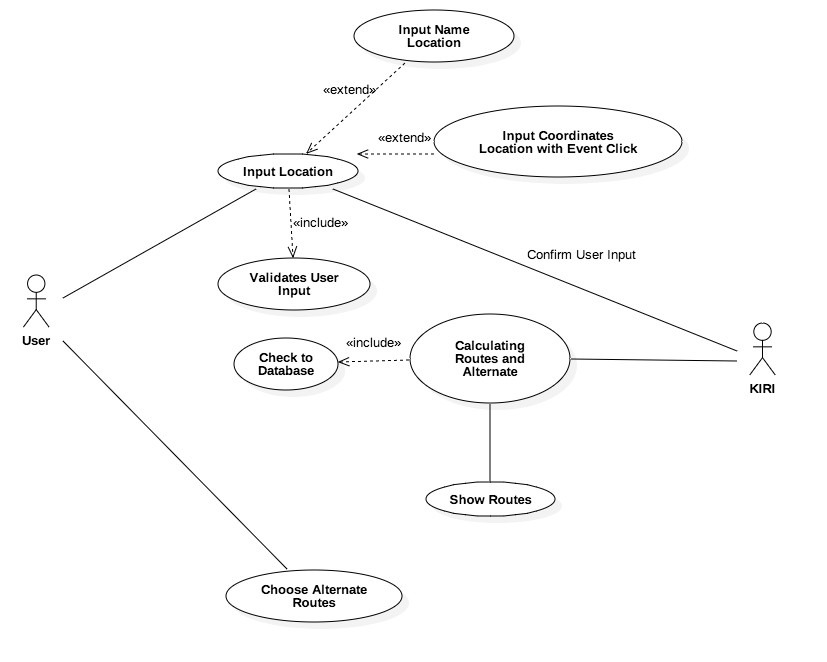
\includegraphics[scale=0.5]{Gambar/usecase}
	\caption{Use Case Diagram KIRI} 
	\label{fig:3_usecase}
\end{figure}

Terdapat empat \textit{use case}, yaitu:
\begin{enumerate}
	\item \textbf{Memasukkan lokasi}, pengguna dapat memasukkan lokasi dengan memasukkan nama lokasi ataupun melakukan klik pada peta dan diubah menjadi koordinat.
	\item \textbf{Memilih rute alternatif}, pengguna dapat memilih rute alternatif (jika ada) setelah proses pencarian rute.
	\item \textbf{Mengganti bahasa}, pengguna dapat memilih bahasa yang ingin digunakan dengan bahasa yang disediakan, Bahasa Indonesia atau Bahasa Inggris.
	\item \textbf{Mengganti lokasi kota}, pengguna dapat memilih lokasi kota mana yang ingin digunakan dengan pilihan kota yang disediakan, yaitu: Bandung, Jakarta, Surabaya, dan Malang.
	
\end{enumerate}

\subsection{Skenario Use Case}
\begin{enumerate}
	\item \textbf{Memasukkan lokasi}
	\begin{itemize}
			\item Nama: Memasukkan lokasi
			\item Aktor: Pengguna
			\item Deskripsi: Memasukkan lokasi dengan memasukkan nama lokasi ataupun melakukan klik pada peta dan diubah menjadi koordinat.
			\item Kondisi awal: -
			\item Kondisi akhir: Pencarian rute dan rute alternatif (jika ada) yang akan ditampilkan pada pengguna berupa rute pada peta dan penjelasan rute.
			\item Skenario utama: \\ \\
				\begin{tabular}{|p{0.5cm} |p{6cm}| p{6cm}|}
						\hline
							No 	& Aksi Aktor & Reaksi Sistem \\ \hline
							1 	& Pengguna memasukkan lokasi 	&	Sistem mendapatkan lokasi kemudian menampilkan hasil pencarian rute \\ \hline 
						\end{tabular} 
			\item Eksepsi: Lokasi tidak ditemukan.
		\end{itemize}
	\item \textbf{Memilih rute alternatif}
	\begin{itemize}
			\item Nama: Memilih rute alternatif
			\item Aktor: Pengguna
			\item Deskripsi: Memilih rute alternatif.
			\item Kondisi awal: Pencarian rute sudah berhasil dan ada rute alternatif
			\item Kondisi akhir: Menampilkan kepada pengguna rute alternatif pada peta beserta penjelasannya.
			\item Skenario utama: \\ \\
				\begin{tabular}{|p{0.5cm} |p{6cm}| p{6cm}|}
						\hline
							No 	& Aksi Aktor & Reaksi Sistem \\ \hline
							1 	& Pengguna memilih rute alternatif 	&	Sistem menampilkan pencarian rute alternatif pada peta dan penjelasannya \\ \hline 
						\end{tabular} 
			\item Eksepsi: Tidak ada rute alternatif.
		\end{itemize}
	\item \textbf{Mengganti bahasa}
	\begin{itemize}
			\item Nama: Mengganti bahasa
			\item Aktor: Pengguna
			\item Deskripsi: Memilih opsi bahasa yang akan digunakan.
			\item Kondisi awal: -
			\item Kondisi akhir: Menampilkan kepada pengguna dengan bahasa yang dipilih
			\item Skenario utama: \\ \\
				\begin{tabular}{|p{0.5cm} |p{6cm}| p{6cm}|}
						\hline
							No 	& Aksi Aktor & Reaksi Sistem \\ \hline
							1 	& Pengguna memilih opsi bahasa 	&	Sistem menampilkan tampilan dengan bahasa yang dipilih oleh pengguna \\ \hline 
						\end{tabular} 
			\item Eksepsi: -
		\end{itemize}
	\item \textbf{Mengganti lokasi kota}
	\begin{itemize}
			\item Nama: Mengganti lokasi kota
			\item Aktor: Pengguna
			\item Deskripsi: Memilih opsi lokasi kota yang akan ditampilkan pada peta dan pencarian rute pada kota tersebut.
			\item Kondisi awal: -
			\item Kondisi akhir: Menampilkan kepada pengguna dengan lokasi kota yang dipilih
			\item Skenario utama: \\ \\
				\begin{tabular}{|p{0.5cm} |p{6cm}| p{6cm}|}
						\hline
							No 	& Aksi Aktor & Reaksi Sistem \\ \hline
							1 	& Pengguna memilih opsi lokasi kota 	&	Sistem menampilkan peta dengan lokasi kota yang dipilih dan menyiapkan pencarian rute pada kota tersebut \\ \hline 
						\end{tabular} 
			\item Eksepsi: -
		\end{itemize}
\end{enumerate}


\section{Analisis Activity Diagram}
\label{sec:activitydiagram}
Diagram aktivitas KIRI dapat dilihat pada \ref{fig:3_activitydiagram}.

\begin{figure}[H]
	\centering
	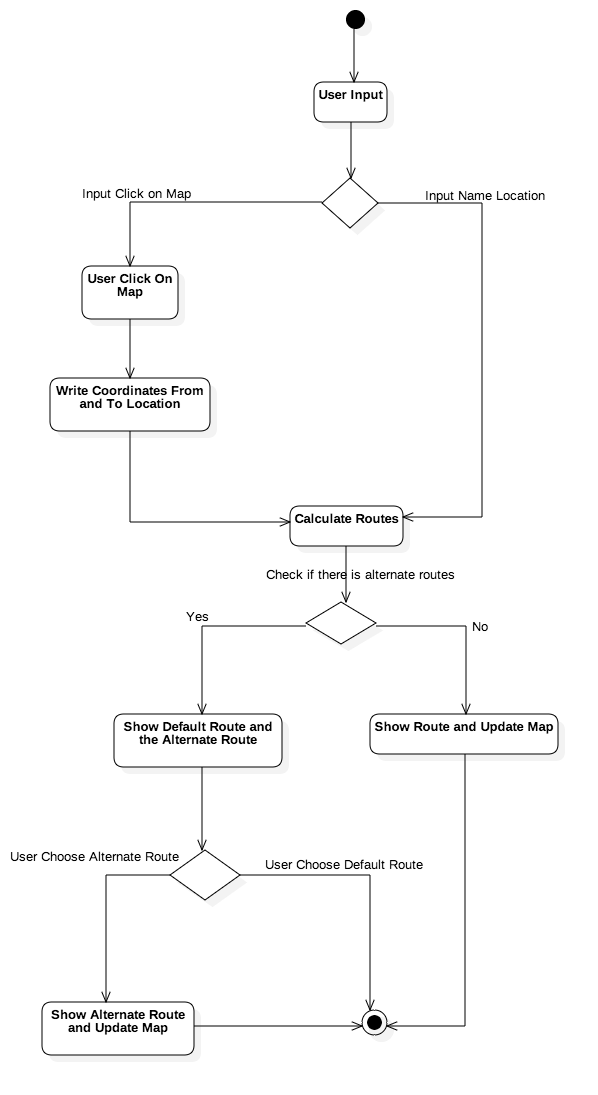
\includegraphics[scale=0.5]{Gambar/activitydiagram}
	\caption{Activity Diagram KIRI} 
	\label{fig:3_activitydiagram}
\end{figure}

Aktivitas-aktivitas yang ada pada KIRI dapat dijelaskan sebagai berikut:

\begin{enumerate}
	\item Pengguna memberikan masukan. Masukan dapat berupa dua, yaitu:
	\begin{itemize}
		\item Masukan berupa nama lokasi.
		\item Masukan berupa klik pada peta. Pengguna klik pada peta, kemudian sistem mendapatkan koordinat pada lokasi yang diklik pengguna dan menulis koordinat tersebut kepada \textit{textfield} tempat asal atau tujuan.
	\end{itemize}
	\item Sistem melakukan proses pencarian rute dan melakukan pengecekan apakah ada rute alternatif atau tidak.
	\begin{itemize}
		\item Jika tidak ada rute alternatif, maka menunjukkan rute dan memperbarui peta.
		\item Jika ada rute alternatif, menunjukkan pada pengguna rute \textit{default} dan rute alternatif.
	\end{itemize}
	\item Pengguna memilih rute default atau rute alternatif.
	\begin{itemize}
		\item Jika pengguna memilih rute default, aktivitas selesai.
		\item Jika pengguna memilih rute alternatif, maka sistem menunjukkan rute alternatif dan memperbarui peta.
	\end{itemize}
\end{enumerate}